\chapter{Xử lý Dữ liệu}

Chương này trình bày chi tiết các bộ dữ liệu, lược đồ chuẩn hóa, quy trình làm sạch, kỹ thuật tạo đặc trưng và tiền xử lý tín hiệu âm thanh phục vụ đồng thời cả \texttt{Retail-AI-} và \texttt{ops\_chest}.

\section{Mô tả Dữ liệu}

Trên toàn nền tảng tác nhân kép, sáu bộ dữ liệu và tập kiểm chuẩn thực nghiệm được tổ chức rõ ràng cho việc neo danh mục sản phẩm, kiểm thử chống nhiễu giọng nói, đánh giá an toàn và tối ưu nhu cầu hàng tươi sống.

\textbf{Bản chụp Danh mục Siêu thị Thanh Lam Mart (\texttt{Retail-AI-}).}
Thu thập ngày 15/09/2026 và lưu tại \code{data/thanh_lam_products.csv} cùng bản chỉ mục JSON \code{data/thanh_lam_products.json}~\cite{thanh_lam_snapshot}, bộ dữ liệu gồm \textbf{3.099 SKU thô} trải rộng trên \textbf{699 thương hiệu} và \textbf{346 đường dẫn ngành hàng phân cấp} (đồ uống, sữa, thịt tươi, thực phẩm khô, chăm sóc cá nhân, hóa phẩm giặt tẩy và đồ gia dụng). Mỗi bản ghi lõi gồm 20 trường cấu trúc (mã SKU, tên sản phẩm chuẩn hóa Việt/Anh, thương hiệu, giá niêm yết, giá khuyến mãi, nội dung ưu đãi, đơn vị tính, quy cách đóng gói và cây ngành hàng). Mười hai trường thống kê mở rộng (số lượng bán 30 ngày, doanh thu, đánh giá, nhãn bán chạy) được tách biệt chủ đích sang \code{data/demo_sales.sqlite3} và gắn nhãn \texttt{SIMULATED} để dữ liệu minh họa không bao giờ bị nhầm với lịch sử POS thực tế.

\textbf{Bộ Kiểm chuẩn SOTA~V2 và Tập Tiếng nói Siêu thị Nhiều Mức Nhiễu (\texttt{Retail-AI-}).}
Để đánh giá khả năng tổng quát hóa mà không học tủ unit test, nhóm xây dựng bộ 100 câu hỏi tiếng Việt và song ngữ chưa từng thấy (113 lượt hội thoại phủ 10 nhóm: tra cứu trực tiếp, đa thuộc tính, giỏ hàng ngân sách, so sánh, khuyến mãi, an toàn y tế/lâm sàng, phương ngữ/lỗi nhận dạng, câu hỏi vô hại XSTest, tấn công tiêm lệnh red-team OWASP và nhất quán diễn đạt tương đương). Đánh giá âm học kết hợp 8 đoạn giọng người Việt sạch và 8 câu lệnh thương hiệu Thanh Lam Mart dưới 3 mức SNR (sạch, nhiễu siêu thị 12\,dB và nhiễu nặng 5\,dB), cùng 10 truy vấn thực tế đo độ trễ streaming đầu-cuối.

\textbf{Bộ Dữ liệu Nhu cầu Hàng Tươi sống Thực FreshRetailNet-50K (\texttt{ops\_chest}).}
Nhu cầu vận hành hậu cần được hiệu chuẩn trên bộ dữ liệu công khai \emph{FreshRetailNet-50K} (\code{Dingdong-Inc/FreshRetailNet-50K}, giấy phép CC BY 4.0)~\cite{freshretailnet50k}, ghi nhận lượng bán theo giờ và cờ đứt hàng tại các cửa hàng tiện lợi thực tế. \texttt{ops\_chest} sử dụng \textbf{50 cửa hàng kiểm định độc lập} (2.675 chuỗi thời gian SKU--cửa hàng) cho huấn luyện, đánh giá ML ngoài mẫu và backtest lợi nhuận từ 28/03/2024 đến 02/07/2024 (90 ngày lịch sử đến mốc cắt $T_{\text{cut}} = \text{25/06/2024}$, mốc khởi đầu backtest $T_0 = \text{26/05/2024}$ và tuần đánh giá 7 ngày). \textbf{Cửa hàng mẫu số 18} đóng vai trò môi trường vận hành tương tác với \textbf{164 SKU tươi sống} trong 90 ngày. Vì FreshRetailNet-50K ẩn danh tên hàng và không kèm giá bán/hợp đồng nhà cung cấp, mô-đun \code{frn_catalog.py} gán xác định tên hiển thị trung tính, giá bán (12.000--80.000\,VND), tỷ lệ giá vốn (62--75\%), hạn dùng 1--3 ngày, nhà cung cấp giả lập (\texttt{*.test}) và cờ top-5 mặt hàng hút khách. Một môi trường tổng hợp phụ 263 SKU $\times$ 365 ngày (\code{--source synthetic}) được giữ riêng để chạy kiểm thử đơn vị cho các quy tắc nghiệp vụ.

\begin{table}[H]
\centering
\caption{Thống kê các bộ dữ liệu và tập kiểm chuẩn sử dụng trên cả hai kho mã nguồn}
\label{tab:dataset_stats}
\footnotesize
\begin{tabularx}{\textwidth}{L{3.5cm} L{2.2cm} L{3.6cm} Y}
\toprule
\textbf{Bộ dữ liệu / Tập kiểm thử} & \textbf{Phân hệ} & \textbf{Quy mô / Phân chia} & \textbf{Vai trò \& Nguồn gốc} \\
\midrule
Danh mục Thanh Lam Mart (\code{thanh_lam_products}) & \texttt{Retail-AI-} & 3.099 SKU thô (3.081 hợp lệ, 18 cách ly); 699 thương hiệu; 346 nhánh ngành; 3.096 ảnh & Cơ sở dữ liệu gốc cho tìm kiếm, đơn giá quy đổi, popup ảnh sản phẩm và khuyến mãi (15/09/2026) \\
Kho Tri thức Sản phẩm Đa nguồn (\code{thanh_lam_product_details} + pilot) & \texttt{Retail-AI-} & 2.137/3.099 SKU sạch (1.214+18 thành phần, 1.064+ chi tiết, 1.159 HDSD, 660 bảo quản, 800 xuất xứ) & Crawl SSR Thanh Lam Mart + đối chiếu mã vạch EAN-13/nhãn Kingfoodmart \& Long Châu; qua 8 tầng làm sạch đạt \textbf{0 lỗi QA} \\
Dữ liệu bán thử (\code{demo_sales.sqlite3}) & \texttt{Retail-AI-} & Lượt bán 30 ngày của 3.099 SKU & Xếp hạng bán chạy xác định tách biệt (hỗ trợ khẩu ngữ), luôn gắn nhãn \texttt{SIMULATED} \\
Tập SOTA~V2, 100Q Chuyên gia \& Audit Production & \texttt{Retail-AI-} & 100 câu SOTA~V2 (113 lượt) + 100 câu danh mục mới + 12 câu live \texttt{sin1} & Đo độ chính xác, 5 chuẩn SOTA (RAGAS/DeepEval/RAGChecker/$\tau$-bench), TTFT \& bộ đệm ngữ nghĩa \\
Tập Tiếng nói Đa Mức SNR & \texttt{Retail-AI-} & 8 mẫu người thật + 8 mẫu thương hiệu $\times$ 3 mức SNR (Sạch, 12\,dB, 5\,dB) & So sánh WER 5 cấu hình STT, khử nhiễu nơ-ron và trễ WebSocket \\
FreshRetailNet-50K (\code{frn})~\cite{freshretailnet50k} & \texttt{ops\_chest} & 50 cửa hàng (2.675 chuỗi); Cửa hàng 18: 164 SKU $\times$ 90 ngày; 200k kiểm tra khôi phục & Hiệu chuẩn nhu cầu tươi sống thực, LightGBM~v3 phân vị và backtest lợi nhuận 37 ngày \\
Cửa hàng Tổng hợp (\code{--source synthetic}) & \texttt{ops\_chest} & 263 SKU $\times$ 365 ngày & Unit test xác định cho FEFO, trả hàng NCC, kiểm kê mù và HITL \\
\bottomrule
\end{tabularx}
\end{table}

\subsection*{Trực quan hóa Dữ liệu Danh mục}
Hình~\ref{fig:thanh_lam_dist} minh họa phân bố top-10 nhóm ngành hàng và phân bố giá bán tham khảo của 3.099 SKU Thanh Lam Mart, cho thấy mật độ mã hàng tập trung mạnh ở các ngành hàng tiêu dùng thiết yếu hằng ngày và phân bố giá lệch phải tập trung quanh ngưỡng 35.000--45.000\,VND.

\begin{figure}[H]
    \centering
    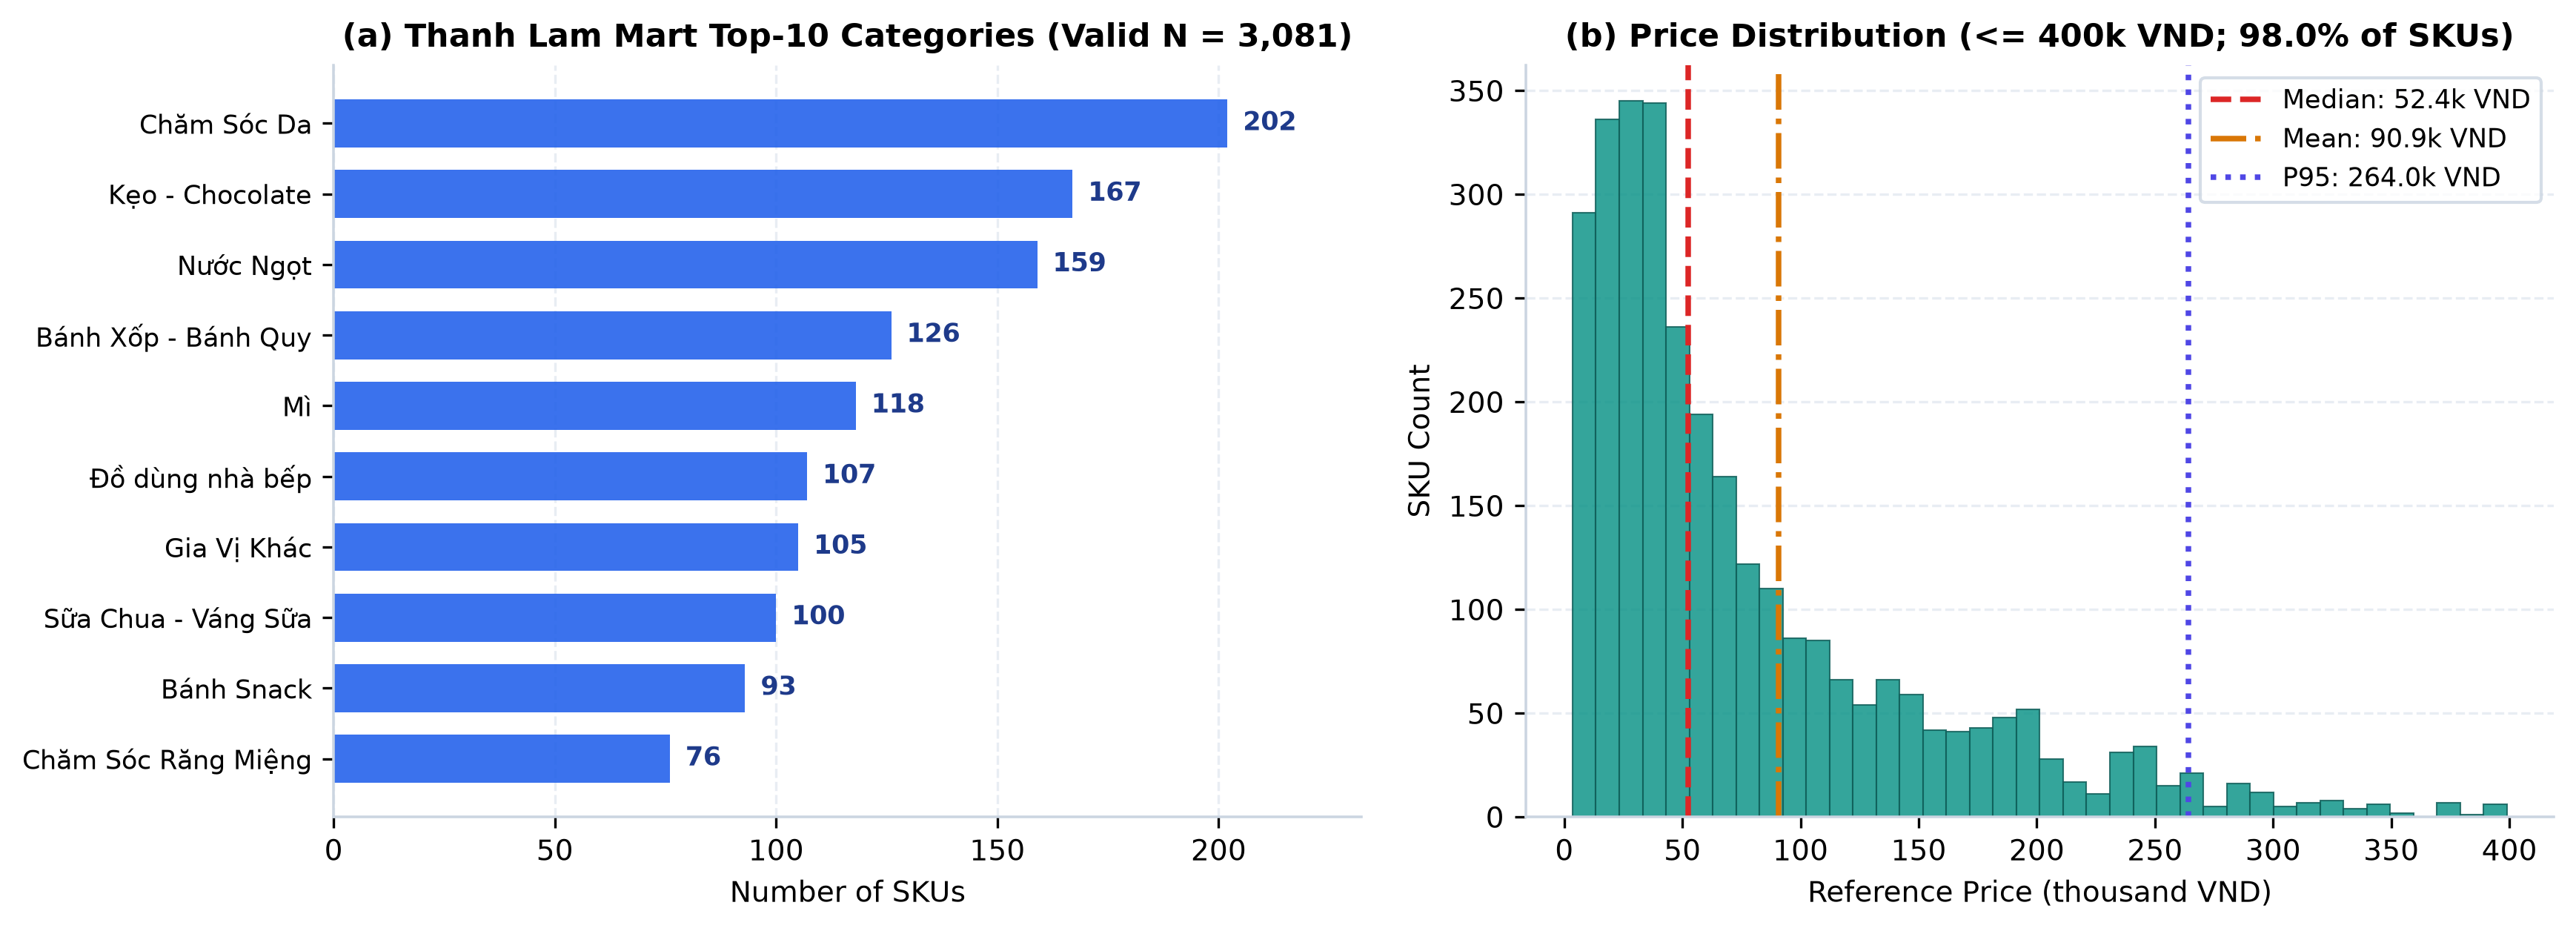
\includegraphics[width=0.98\textwidth]{Images/fig_catalog_distribution.png}
    \caption{Phân bố top-10 ngành hàng (trái) và phân bố giá tham khảo (phải) của bản chụp danh mục Thanh Lam Mart ($N = 3.099$ SKU).}
    \label{fig:thanh_lam_dist}
\end{figure}

\section{Tiền xử lý và Làm sạch Dữ liệu}

\subsection*{Cách ly Lỗi Lược đồ và Chuẩn hóa Từ vựng Danh mục (\texttt{Retail-AI-})}
Mọi bản ghi nạp vào \texttt{Retail-AI-} đều đi qua lớp kiểm định Pydantic chặt chẽ (\code{ThanhLamRow}):
\begin{enumerate}
    \item \textbf{Cách ly bất thường giá:} 18 trong số 3.099 dòng thô (0,58\%) bị lỗi giá khuyến mãi cao hơn giá niêm yết; bộ nạp tự động cách ly 18 bản ghi này và đưa 3.081 SKU hợp lệ (99,42\%) vào danh mục truy xuất.
    \item \textbf{Đánh chỉ mục không dấu và đồng nghĩa:} Tên sản phẩm, thương hiệu và đường dẫn ngành hàng được chuẩn hóa Unicode NFC và lược bỏ dấu tiếng Việt (\code{normalize_category_text}) để dựng bảng chỉ mục đảo sẵn trong \code{SnapshotProductRepository}, rút ngắn tốc độ truy xuất từ $3{,}7\times$ đến $4{,}5\times$.
    \item \textbf{Trích xuất định lượng và thuộc tính:} Biểu thức chính quy bóc tách trọng lượng/thể tích/quy cách (g, kg, ml, L, gói, lốc, thùng) phục vụ quy đổi đơn giá chuẩn (Công thức~\ref{eq:unit_price}), nhãn đường (\emph{không đường}, \emph{ít đường}) và đối tượng sử dụng.
    \item \textbf{Hàng rào sửa lỗi ASR neo theo danh mục:} Do đối sánh mờ thô sơ với 3.099 tên hàng từng làm hỏng từ tiếng Việt thông thường (như biến \emph{``vĩnh viễn''} $\to$ \emph{``MINH viền''}, \emph{``anh em''} $\to$ \emph{``Bánh em''}, \emph{``Campuchia''} $\to$ \emph{``Capuchiano''} và \emph{``Home''} $\to$ \emph{``Wmhome''}), mô-đun \code{catalog_transcription.py} áp dụng danh sách bảo vệ \code{_NEVER_CORRECT} song song với cụm sửa thương hiệu đã kiểm chứng (\emph{Thanh Lam Mart hôn} $\to$ \emph{Thanh Lam Home}, \emph{ACFOGS} $\to$ \emph{ACEFOODS}, \emph{khăn mặt proton} $\to$ \emph{khăn mặt cotton}).
\end{enumerate}

\subsection*{Làm giàu Tri thức Thành phần Đa nguồn và Pipeline Làm sạch 8 Tầng (\texttt{Retail-AI-})}
Vì bản chụp CSV/JSON gốc của Thanh Lam Mart thiếu trường thành phần, hướng dẫn sử dụng và bảo quản, nhóm xây dựng quy trình thu thập và chuẩn hóa tri thức sản phẩm toàn danh mục (\code{scripts/crawl_thanh_lam_product_details.py}, \code{scripts/enrich_detailed_ingredients.py}, \code{scripts/clean_thanh_lam_product_details.py}) gắn chặt mã băm SHA-256 của \code{thanh_lam_products.json} mà không làm thay đổi tệp catalog gốc:
\begin{enumerate}
    \item \textbf{Thu thập toàn bộ 3.099 trang SSR Thanh Lam Mart và đối chiếu nhãn đa nguồn:} Trích xuất dữ liệu \code{__NEXT_DATA__} từ toàn bộ 3.099/3.099 trang Thanh Lam Mart trong 79\,giây, sau đó nâng cấp các SKU thiếu thành phần hoặc chỉ có mô tả tiếp thị chung chung (ví dụ \emph{Tương ớt Chin Su chai 1kg} ban đầu chỉ ghi \emph{``ớt tươi chọn lọc cùng các chất phụ gia''}) bằng cách đối chiếu nguồn nhãn công khai từ \textbf{Kingfoodmart} (10.281 sản phẩm) và \textbf{Nhà thuốc Long Châu} (dược mỹ phẩm \& chăm sóc cá nhân). Cơ chế xác minh hai tầng chỉ chấp nhận \textbf{333 khớp mã vạch EAN-13 chính xác tuyệt đối} (\code{variant.sku == barcode}) và \textbf{226 khớp chặt thương hiệu--dạng bào chế--hương vị} (loại trừ 64 ca nghi vấn lệch dòng/vật liệu như \emph{TH Milk vs.\ Dalat Milk}, \emph{lăn vs.\ xịt khử mùi}, \emph{PVC vs.\ PE}, \emph{sữa thường vs.\ lactose-free}).
    \item \textbf{Pipeline làm sạch 8 tầng chuẩn Hugging Face \code{datatrove}/FineWeb~\cite{hf_datatrove} \& OpenFoodFacts~\cite{openfoodfacts}:} Chuẩn hóa Unicode NFC, loại bỏ ký tự ẩn (\texttt{U+200B}, \texttt{U+00A0}), xóa ngoặc rỗng \code{()} và lỗi OCR; tự động chèn dấu chấm ngăn tách dòng \code{<li>} bị dính mà vẫn bảo vệ cụm danh từ Việt (\emph{Sữa Rửa Mặt}, \emph{Nước Lau Sàn}); cân bằng cặp ngoặc đơn và cắt sạch tại ranh giới câu thay vì cắt cụt \code{...}; tách lỗi tràn chéo trường (\emph{Hướng dẫn sử dụng}/\emph{Bảo quản} lẫn vào \emph{Thành phần}); cách ly 100\% rác OCR ngoại ngữ và các tuyên bố dị ứng chưa xác minh có rủi ro an toàn thực phẩm (như chuỗi \emph{``NO MILK. SAFE FOR MILK ALLERGIES''} trên bánh quy Oreo); giữ chuẩn danh pháp mỹ phẩm INCI; và áp dụng \textbf{bộ lọc thực thể có ranh giới từ (word-boundary regex)} kiểm tra vế sau cụm \emph{``làm từ/làm bằng''} để loại bỏ triệt để các câu sáo rỗng lặp tên hàng, câu cụt (\emph{``Có trong bánh...''}) cũng như giả dương tính từ ghép (như \emph{``sả''} trong \emph{``sản phẩm''} hay \emph{``tiêu''} trong \emph{``tiêu chí''}).
    \item \textbf{Kiến trúc 3 tầng ưu tiên bằng chứng (\code{backend/products/knowledge.py}):} Tại thời điểm chạy, hệ thống luôn tuân thủ thứ tự ưu tiên bất biến \texttt{SOURCE\_RECORD} $>$ \texttt{MANUFACTURER\_DECLARATION} (18 SKU công bố hãng chuẩn trong \code{product_knowledge_enrichment_pilot.json}) $>$ \texttt{RETAILER\_LISTING} (\code{thanh_lam_product_details.json}, luôn trích nguồn minh bạch và nhắc khách xem bao bì), và tự động hạ về \texttt{UNKNOWN} với sản phẩm chưa có bảng thành phần xác thực. Kết quả đưa toàn bộ \textbf{4.606 lỗi trên 11 tiêu chí xuống còn 0 lỗi (sạch 100\%)}, nâng tổng độ phủ lên \textbf{2.137/3.099 SKU (69,0\%)} với \textbf{1.214 + 18 SKU} có thành phần sạch (\textbf{1.064+} bảng thành phần định lượng/INCI chi tiết, tăng $2{,}1\times$ so với bản crawl thô Thanh Lam Mart), \textbf{1.159} hướng dẫn sử dụng, \textbf{660} hướng dẫn bảo quản và \textbf{800} xuất xứ (Hình~\ref{fig:catalog_enrichment_cleaning}).
\end{enumerate}

\begin{figure}[H]
    \centering
    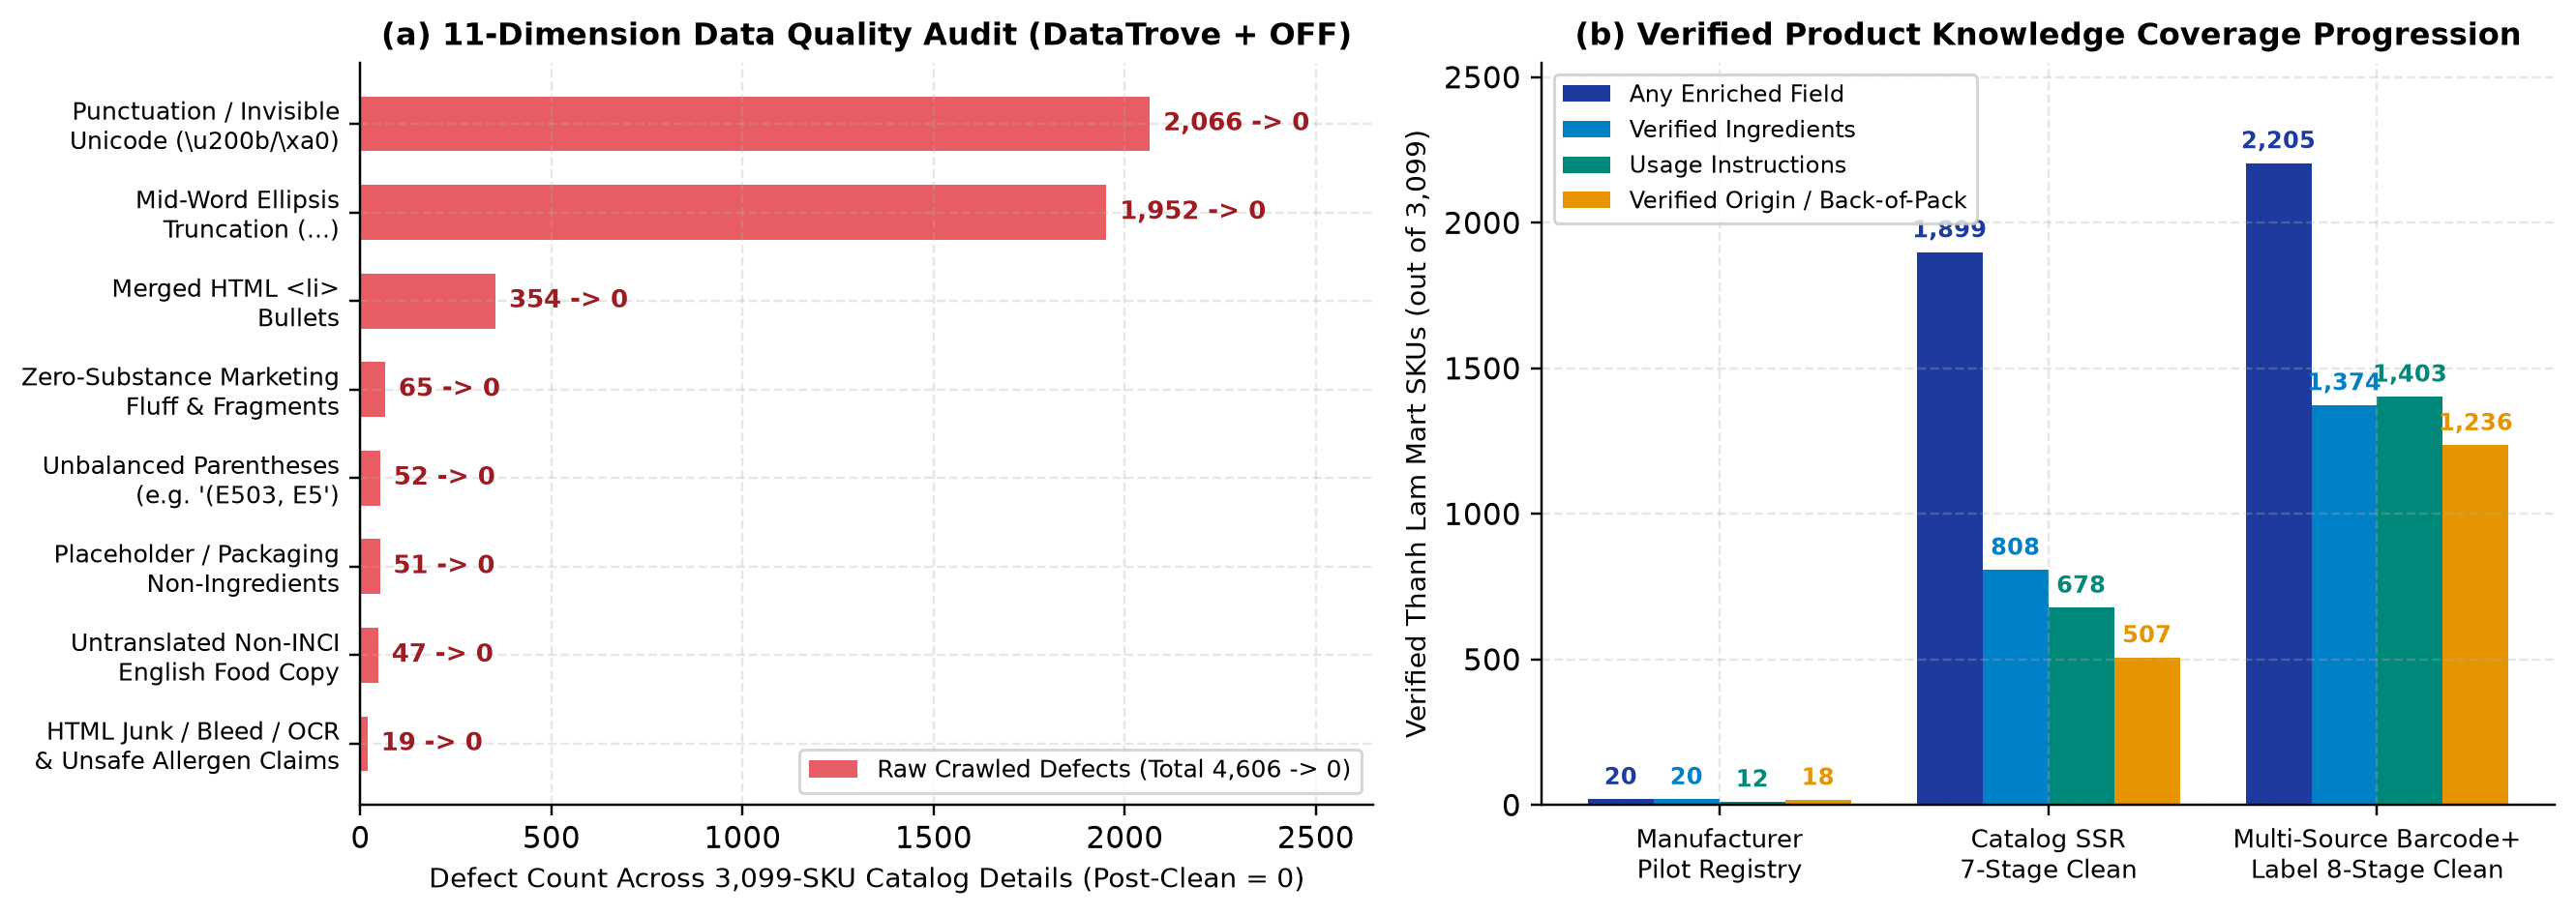
\includegraphics[width=0.98\textwidth]{Images/fig_catalog_enrichment_cleaning.png}
    \caption{Kiểm toán loại bỏ 4.606 lỗi trên 11 tiêu chí về 0 bằng pipeline làm sạch 8 tầng (trái) và tăng trưởng độ phủ tri thức sản phẩm đã xác minh qua các giai đoạn làm giàu đa nguồn (phải).}
    \label{fig:catalog_enrichment_cleaning}
\end{figure}

\subsection*{Tiền xử lý Âm thanh và Tăng cường Tiếng nói (\texttt{Retail-AI-})}
AudioWorklet trên trình duyệt thu tín hiệu đơn kênh 16\,kHz dạng Float32 theo từng khung 32\,ms (512 mẫu) với AEC, AGC và lọc nhiễu phần cứng. Trên luồng WebSocket, bộ đệm vòng 8 khung (256\,ms) giữ trọn phụ âm đầu của tiếng Việt rồi chuyển sang PCM16 có dấu. Trên luồng REST/cứu hộ (\code{speech_activity.py}, \code{speech_denoiser.py}), đoạn âm thanh được giải mã bằng PyAV về 16\,kHz, cắt gọn theo biên tiếng nói Silero VAD~v6 (đệm $\pm 180/200$\,ms), qua bộ lọc thông cao 85\,Hz (Công thức~\ref{eq:hpf85}) và khử nhiễu có điều kiện bằng \texttt{DPDFNet2} ONNX theo Công thức~\ref{eq:snr_blend}.

\subsection*{Khôi phục Nhu cầu Đứt hàng và Tạo 29 Đặc trưng (\texttt{ops\_chest})}
Trong \texttt{ops\_chest} (\code{ml_features.py} và \code{forecast.py}), dữ liệu bán hàng thô FreshRetailNet trải qua ba bước tiền xử lý cốt lõi trước khi huấn luyện LightGBM phân vị:
\begin{enumerate}
    \item \textbf{Khôi phục nhu cầu bị che khuất theo giờ:} Thử nghiệm che các khung giờ cuối ngày trên 200.000 ngày đủ hàng xác nhận việc dùng trực tiếp doanh số thô gây sai số WAPE 32,3\% và thiên lệch âm $-32{,}3\%$, trong khi khôi phục theo hồ sơ giờ (Công thức~\ref{eq:wape_recovery}) hạ WAPE còn \textbf{20,5\%} và gần như triệt tiêu thiên lệch (\textbf{$-0{,}1\%$}).
    \item \textbf{Quy đổi hệ số đơn vị và điền khuyết ngày đứt hàng:} Sản lượng FreshRetailNet được nhân hệ số $K = 10$ để SKU trung vị đạt khoảng 7 đơn vị/ngày (đảm bảo sàn phương sai Poisson thực tế cho EWMA), và các ngày đứt hàng quá khứ được điền bằng trung bình cùng thứ trong tuần trước khi tính đặc trưng trễ.
    \item \textbf{Xây dựng 29 đặc trưng dạng bảng:} Với mỗi chân trời dự báo $h \in \{1,\dots,7\}$, hàm \code{build_features} tạo 29 đặc trưng: 7 độ trễ ngày (\code{lag1}--\code{lag7}), trung bình trượt (\code{mean3}, \code{mean7}, \code{mean14}), cùng thứ trong tuần (\code{same_wd}, \code{same_wd_last}), độ phân tán và tính gián đoạn 28 ngày (\code{std28}, \code{zero28}), lịch sử đứt hàng (\code{stockout28}, \code{stockout7}, \code{days_since_stockout}, \code{stockout_last}), xu hướng và mức log, điểm neo EWMA 56 ngày (\code{ewma_h}, \code{ewma_sigma}), biến lịch/chân trời (\code{h}, \code{target_wd}, \code{origin_wd}, \code{target_holiday}) và phân cấp ngành hàng (\code{mgmt_group}, \code{cat1}, \code{cat2}). Đặc biệt, đặc trưng giảm giá ngày mục tiêu đã bị loại bỏ sau khi phiên bản v1 cho thấy giả định không giảm giá tương lai gây thiên lệch dự báo thấp $-15{,}7\%$, còn phép hiệu chỉnh độ co giãn giá ($e \approx 9{,}6$) ở v2 bị loại bỏ do gây lệch 14--31\%; phiên bản v3 huấn luyện trực tiếp trên nhu cầu đã khôi phục neo vào đặc trưng EWMA.
\end{enumerate}

\section{Tổng kết Xử lý Dữ liệu}

Cả hai quy trình xử lý dữ liệu đều thực thi nguyên tắc tách bạch nghiêm ngặt giữa \emph{sự thật đã kiểm chứng} và \emph{giả định vận hành có tài liệu hóa}. Ở tuyến trước, 3.081 SKU Thanh Lam Mart sạch, kho tri thức 2.137 SKU đã qua 8 tầng làm sạch đạt 0 lỗi (1.214+18 SKU có thành phần đã xác minh, 3.096 SKU có URL ảnh hợp lệ), bộ phân tích đơn giá xác định và từ vựng bảo vệ ASR mang lại điểm neo chính xác tuyệt đối cho tác nhân kiosk. Ở tuyến sau, khôi phục nhu cầu theo giờ và 29 đặc trưng bảng biến nhật ký FreshRetailNet-50K thành dữ liệu không thiên lệch cho dự báo phân vị và backtest cổng lợi nhuận. Những thiếu hụt dữ liệu còn lại---khoảng 59\% SKU chưa có bảng thành phần định lượng hoặc calo công khai và giả định giá vốn/hạn dùng trong FreshRetailNet---đều được kiểm soát bằng ranh giới an toàn fail-closed tại thời điểm chạy thay vì che giấu bằng suy đoán của LLM.
